\appendix
\addcontentsline{toc}{part}{ХАВСРАЛТ}

\chapter{Ирмэг илрүүлэгч}
\label{appendix:get_edges}

\begin{lstlisting}[language=Python]
@classmethod
def get_edges(cls, source):
		# _THRESHOLD_MIN: 100, _THRESHOLD_MAX: 200
		return cv.Canny(source, cls._THRESHOLD_MIN, cls._THRESHOLD_MAX) 
\end{lstlisting}

\chapter{Хүснэгт илрүүрэгч}
\label{appendix:get_container}

\begin{lstlisting}[language=Python]
@classmethod
def get_form_container(cls, source):
		contours, _ = cv.findContours(
				cls.get_edges(source),
				cv.RETR_EXTERNAL,
				cv.CHAIN_APPROX_SIMPLE,
		)
		biggest_contour = sorted(
				contours,
				key=lambda contour: cv.arcLength(contour, True),
				reverse=True,
		)[0]
		x, y, w, h = cv.boundingRect(biggest_contour)
		bounding_rect_points = rectangle2points(x, y, w, h)
		approx_curve = cv.approxPolyDP(
				biggest_contour,
				0.01 * cv.arcLength(biggest_contour, True),
				True,
		)

		if len(approx_curve) >= 4:
				points = tuple(
						(
								point[0][0] + point[0][1],
								point[0][0] - point[0][1],
								(point[0][0], point[0][1]),
						)
						for point in approx_curve
				)
				sum_sorted_points = sorted(
						points, key=lambda point: point[0]
				)
				diff_sorted_points = sorted(
						points, key=lambda point: point[1]
				)

				extreme_points = (
						sum_sorted_points[0][-1],
						diff_sorted_points[-1][-1],
						diff_sorted_points[0][-1],
						sum_sorted_points[-1][-1],
				)

				homog, _ = cv.findHomography(
						np.array(extreme_points),
						np.array(bounding_rect_points),
				)
				transformed = cv.warpPerspective(
						source,
						homog,
						(int(source.shape[1]), int(source.shape[0])),
				)
				new_x, new_y, new_w, new_h = cls.compensate(
						x, y, w, h, offset=5
				)
				return transformed[
						new_y : new_y + new_h, new_x : new_x + new_w
				]
		return None
\end{lstlisting}

\chapter{Тэмдэгтүүдийг салгах}
\label{appendix:get_chars}

\begin{lstlisting}[language=Python]
@classmethod
def get_characters(cls, form, label_seq: str, skip_char: str):
		h, w, _ = form.shape
		height = (h + (10 - int(str(h)[-1]))) // 10
		width = (w + (10 - int(str(w)[-1]))) // 10
		label_height = height - width
		character_seq = [
				form[
						row * height + label_height : row * height + height,
						col * width : col * width + width,
				]
				for row in range(10)
				for col in range(10)
		]

		return tuple(
				(label, letter)
				for label, letter in zip(label_seq, character_seq)
				if label != skip_char
		)
\end{lstlisting}

\chapter{Тэмдэгт боловсруулах}
\label{appendix:get_char}

\begin{lstlisting}[language=Python]
@classmethod
def get_char(cls, label, source):
		binary = cls.get_threshold(
				cls.get_blurred_img(cls.get_gray_img(source)),
				cv.THRESH_BINARY_INV,
		)
		contours, _ = cv.findContours(
				binary, cv.RETR_EXTERNAL, cv.CHAIN_APPROX_SIMPLE
		)
		sorted_contours = sorted(
				contours,
				key=lambda ctr: cv.contourArea(ctr),
				reverse=True,
		)
		point_x = []
		point_y = []
		for x, y, w, h in (
				cv.boundingRect(ctr) for ctr in sorted_contours
		):
				point_x.append(x)
				point_x.append(x + w)
				point_y.append(y + h)
				point_y.append(y)

		points = list(zip(sorted(point_x), sorted(point_y)))

		if not points:
				return

		max_col = points[-1][0]
		max_row = points[-1][1]
		min_col = points[0][0]
		min_row = points[0][1]

		w_a = max_col - min_col
		h_a = max_row - min_row

		if w_a > h_a:
				diff_x = 0
				diff_y = (w_a - h_a) // 2
		elif w_a < h_a:
				diff_x = (h_a - w_a) // 2
				diff_y = 0
		else:
				diff_x = 0
				diff_y = 0

		diff_x += cls._BORDER_THICKNESS
		diff_y += cls._BORDER_THICKNESS

		cropped = binary[min_row:max_row, min_col:max_col]
		cropped = cv.copyMakeBorder(
				cropped,
				diff_y,
				diff_y,
				diff_x,
				diff_x,
				borderType=cv.BORDER_CONSTANT,
				value=[0, 0, 0],
		)

		if cropped.size != 0:
				resized = cv.resize(
						cropped, cls._SIZE, interpolation=cv.INTER_AREA
				)
				_, final = cls.get_threshold(
						resized, cv.THRESH_BINARY + cv.THRESH_OTSU, 
						adaptive=False
				)
				return final
		return
\end{lstlisting}

\chapter{NUMiner --- Тохиргоог унших}
\label{appendix:handle_config}

\begin{lstlisting}[language=Python]
def handle_config(arg):
		import json
		with open(arg) as config_file:
				config = json.load(config_file)
				Sheet._CHARACTER_SEQUENCE = tuple(config["labels"].items())

		return Sheet._CHARACTER_SEQUENCE
\end{lstlisting}

\newpage
\pagenumbering{gobble}
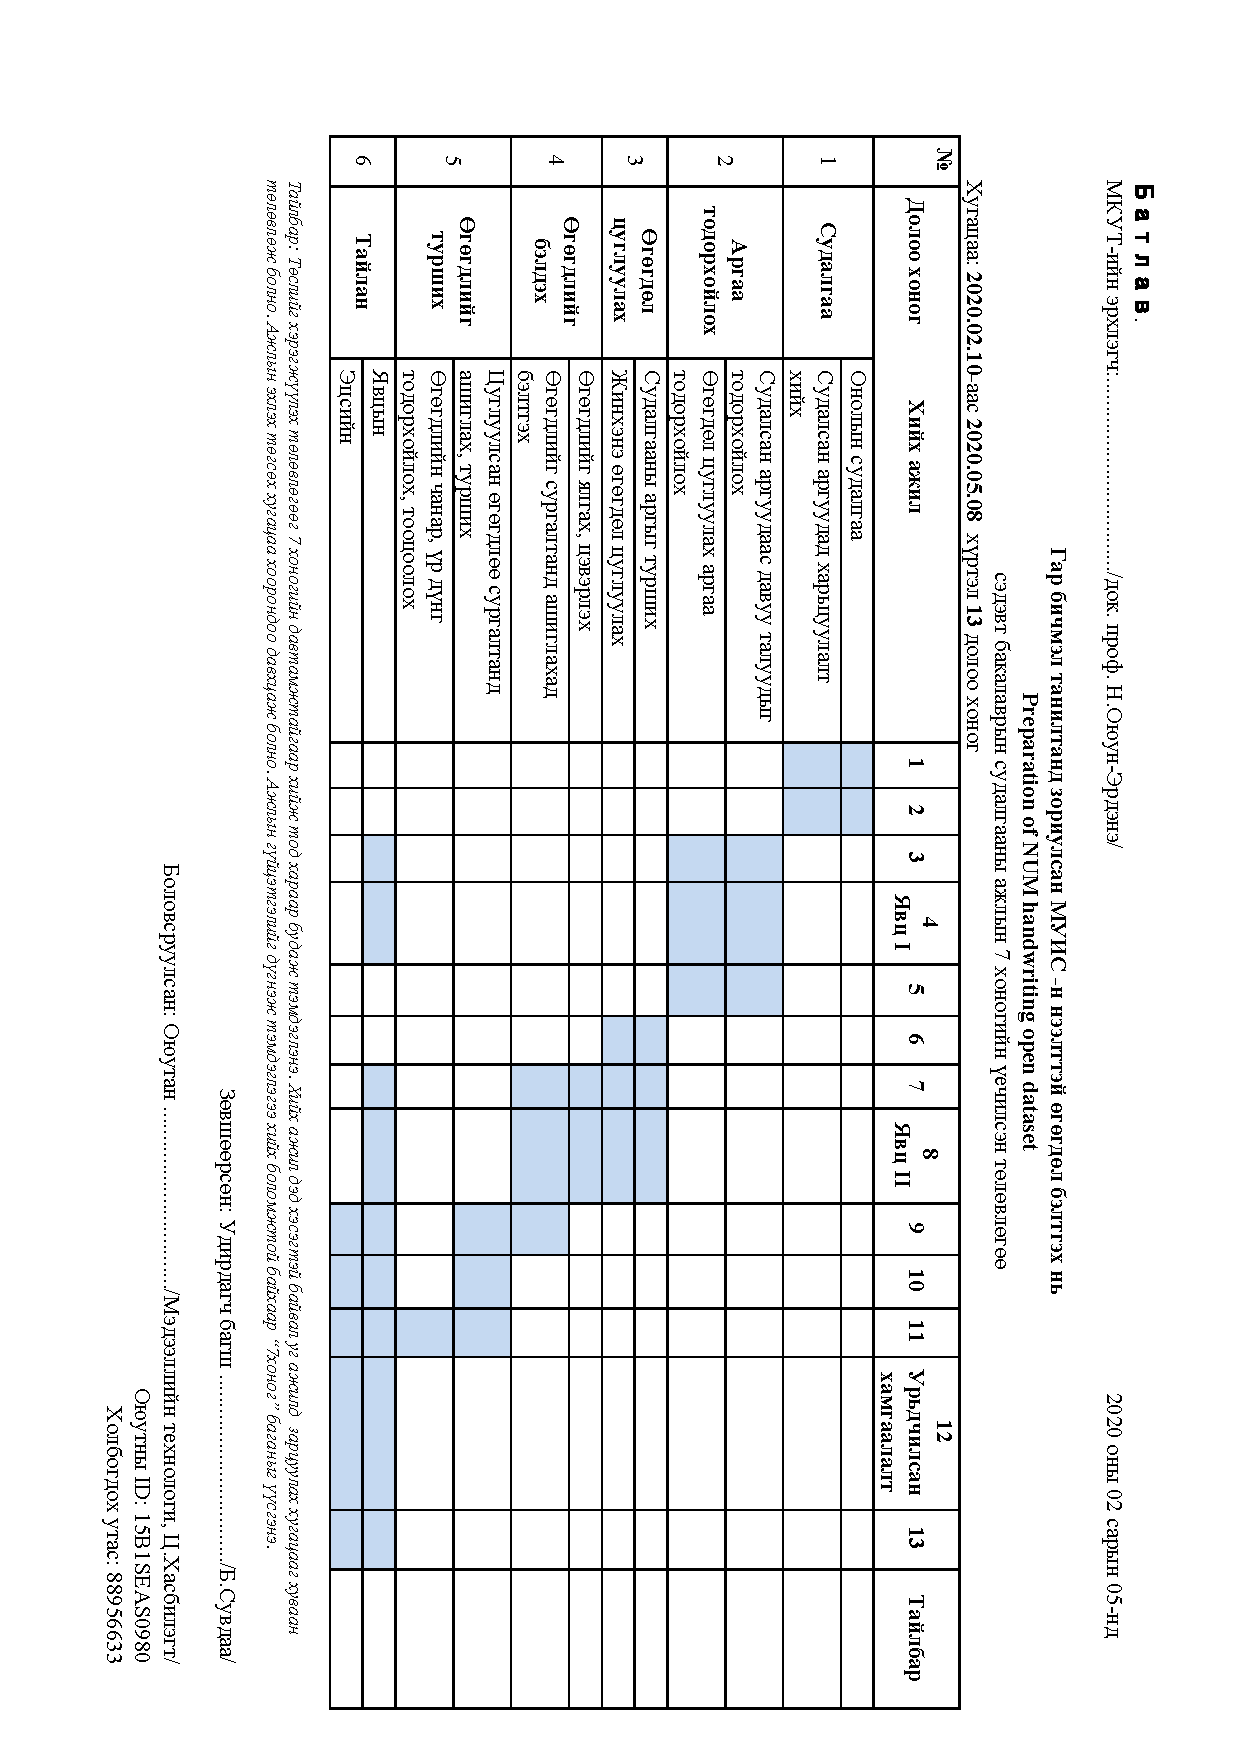
\includepdf[pages=-,pagecommand={},width=\textwidth]{schedule.pdf}
